\chapter{Power Converters}

\begin{pline}
    \item \textbf{PWM}: pulse width modulation is the ratio of the on-time to the off-time
    \item \textbf{PFM}: pulse frequency modulation is a method for generating the equivalent output by changing the frequency (OFF time) while keeping the ON time constant. There is also a type that varies the ON time while keeping the OFF time constant.
    \item \textbf{SMPS}: switched-mode power supplies
\end{pline}

The operation of a power converter can be explained through the following steps:
\begin{enumerate}
    \item \textbf{Energy storage}: Power converters often use inductors and capacitors as energy storage elements. Inductors store energy in the form of a magnetic field when current flows through them, while capacitors store energy in the form of an electric field between their plates.
    \item \textbf{Switching}: The semiconductor switches in the converter turn on and off at high frequencies, which can range from tens of kilohertz to several megahertz, depending on the application. This switching action shapes the flow of energy from the input to the output.
    \item \textbf{Control circuitry}: The switching elements are controlled by a circuit that determines the timing and sequence of their operation. This control circuitry is designed to respond to the input conditions and the desired output specifications. It uses feedback from the output to adjust the switching parameters in real time to maintain the correct output voltage or current.
    \item \textbf{Filtering}: After the switching process, the resulting waveform may contain ripples or high-frequency components that are not suitable for the load. Filters, which are typically composed of inductors and capacitors, smooth out these ripples, producing a more stable and continuous output waveform.
    \item \textbf{Transformation}: During the conversion process, the characteristics of the electrical energy are transformed. For example, in a DC-DC converter, the voltage level is changed while maintaining the direct current nature of the power. In an AC-DC converter (rectifier), the alternating current is converted into direct current, and in a DC-AC converter (inverter), the reverse occurs.
\end{enumerate}

\section{AC to DC Converters}
The simplest AC to DC converters is the half wave rectifier. It uses a single diode to block one half of the AC wave, allowing only one polarity through. The major limitation of a half-wave rectifier is that it utilizes only half of the input waveform. This leads to a low rectification efficiency and high ripple factor, which is the measure of fluctuations in the output DC signal. 

A more efficient design is the full-wave rectifier, which can be implemented in two ways: using a center-tapped transformer with two diodes or using a bridge rectifier with four diodes. The full-wave rectifier allows both halves of the AC waveform to pass but inverts one half, so that both halves move in the same direction, effectively doubling the frequency of the resulting DC signal compared to the half-wave rectifier.

Both types of full-wave rectifiers provide a higher average output voltage and better transformation ratio than a half-wave rectifier. 

To achieve a smoother DC output, rectifiers often incorporate filters. The most common type of filter is the capacitor filter. The capacitor charges up when the voltage rises and discharges when it falls, thus reducing the voltage variations. The filter's performance can be quantified by the ripple factor, defined as the ratio of the ripple voltage to the DC voltage level. Lower ripple factors indicate better filtering.

For applications requiring precise control over the output voltage, AC to DC converters may include a voltage regulator.

\begin{figure}[H]
    \centering
    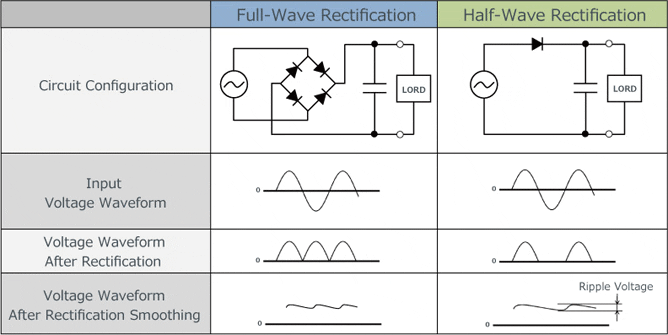
\includegraphics[scale=0.6]{figs/ch03/half_full_wave.png}
\end{figure}

Full-wave rectification rectifies the negative component of the input voltage to a positive voltage, then converts it into DC (pulse current) utilizing a diode bridge configuration. In contrast, half-wave rectification removes just the negative voltage component using a single diode before converting to DC.
Afterward, the waveform is smoothed by charging/discharging a capacitor, resulting in a clean DC signal.
From this, it can be said that full-wave rectification is a more efficient method than half-wave rectification since the entire waveform is used.

Also, a ripple voltage that appears after smoothing will vary depending on the capacitance of this capacitor and the load. Given the same capacitance and load, ripple voltage is smaller with full-wave rectification than haif-wave rectification. Of course it goes without saying that the smaller the ripple voltage the better the stability.

\subsection{Methods}
\begin{enumerate}
    \item \textbf{Transformer method}: This the most common way of performing \textbf{AC-DC conversion}.
    \begin{figure}[H]
        \centering
        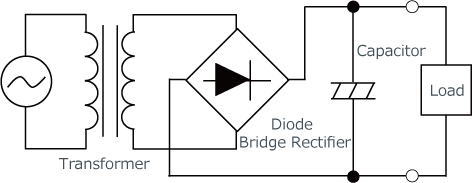
\includegraphics[scale=0.8]{figs/ch03/transformer_ac_dc.png}
        \caption{Input AC voltage is first stepped down to an appropriate level using a transformer and the step-down voltage is set via the winding ratio of the transformer. Then the stepped down AC voltage is full-wave rectified.}
    \end{figure}
    Process is as follows: AC Input $\rightarrow$ Transformer $\rightarrow$ Diode Bridge Rectifier $\rightarrow$ Capacitor

    \item \textbf{Switching method}: 
    \begin{figure}[H]
        \centering
        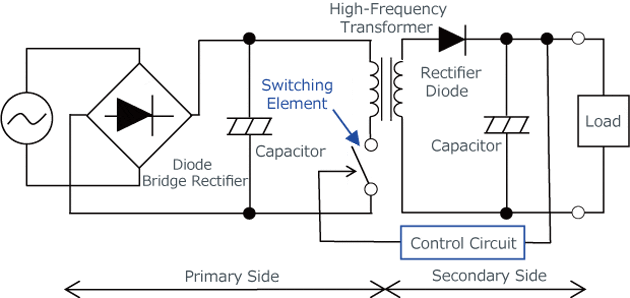
\includegraphics[scale=0.5]{figs/ch03/switching_schematic.png}
        \caption{Transition of the voltage waveform using the switching method.}
        \label{fig:switching_method}
    \end{figure}
    Process is as follows:
    \begin{figure}[H]
        \centering
        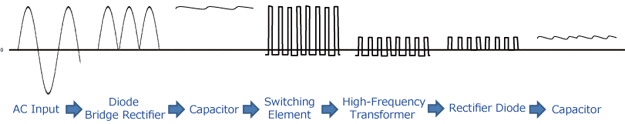
\includegraphics[scale=0.6]{figs/ch03/switching_process.png}
    \end{figure}
    Unlike the transformer method, which first performs step-down AC-AC in the transformer block, with the switching method the input AC voltage is first rectified as-is by the diode bridge circuit. In the case of general households, this input is normally between 100VAC and 200VAC, requiring a diode bridge that can handle large voltages.

    Next the DC waveform is smoothed using a capacitor. Similarly, a high-voltage capacitor is needed.

    Subsequently, this high DC voltage is chopped (separated) by turning ON/OFF the switching element, then transmitted to the secondary side via step-down operation using the high-frequency transformer. At this time, the chopped waveform becomes a square wave.

    The frequency of the switching element is higher than that used in households (i.e. 100kHz vs 50/60kHz). Increasing the frequency allows the use of smaller, lighter transformers.

    On the secondary side, the stepped down square wave is half-wave rectified using a rectifier diode, then smoothed with a capacitor before finally being output as DC voltage.

    In the switching system, a control circuit controls the switching element, making it possible to obtain a stable, predetermined DC output (i.e. 12VDC).

    In contrast to the transformer method, the switching method requires a more complicated circuit configuration utilizing a switching element and control circuit, but high frequency control supports the use of smaller transformers, providing a distinct advantage by reducing set size.

    \item \textbf{Feedback control} is a mechanism for controlling switching elements by checking the output voltage
    \begin{figure}[H]
        \centering
        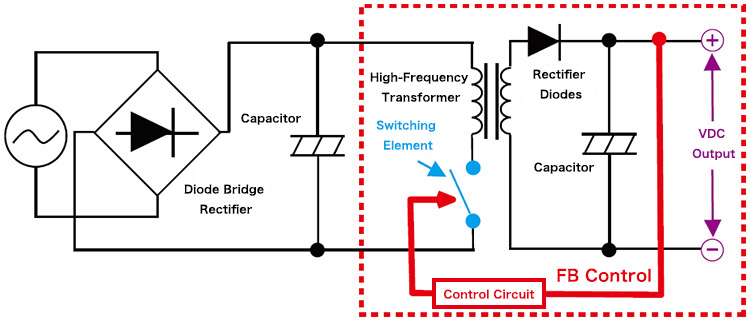
\includegraphics[scale=0.5]{figs/ch03/fb_control.png}
        \caption{This resembles \ref{fig:switching_method}, but we've aded a switching element here with feedback control}
    \end{figure}
    Feedback control helps to see if the actual output voltage matches the predetermined value.
    \begin{enumerate}
        \item Actual output voltage < target value: switching element is controlled so that the ON interval is longer $\rightarrow$ increase the output voltage value.
        \item Actual output voltage > target value: control is carried out so that the ON interval is shorter.
    \end{enumerate}

    \item \textbf{Light load/burst mode}: improves efficiency at light loads (when the output current is small). Switching AC/DC and DC/DC converters supply a stable output voltage by performing chopping via ON/OFF switching then smoothing using a capacitor.
    
    However, momentary current leakage (through-current) is generated during ON/OFF switching. In other words, the more ON/OFF switching operations per unit time, the greater the loss due to leakage current and lower the efficiency. 
    
    When the period is constant (PWM control) the number of switching operations per unit time is constant even if the ON/OFF time ratio changes. Consequently, the (self) power consumption is also constant, resulting in decreased efficiency due to loss caused by leakage current generated during switching at light loads. Therefore, at low current (light load) it is preferable to use PFM control which slows down and lengthens the period, reducing the number of ON/OFF switchings per unit time in order to minimize loss. This technology is called light load mode.

    The PFM method delivers superior efficiency by changing the frequency based on the output current, but noise generated during switching can become irregular. This type of noise, in which the frequency cannot be specified, is difficult to remove, making PWM control featuring a constant frequency more suitable when dealing with noise.

    As such, taking advantage of the trade-off relationship between PWM that minimizes noise and PFM that provides high efficiency by switching to PWM during heavy loads when driving at high frequency (which generates a lot of noise) and PFM at light loads with low current consumption allows users to maximize efficiency throughout the entire load range.
\end{enumerate}

\section{DC to AC Converters}
DC-AC converters are commonly known as \textbf{inverters}. They convert DC from solar panels or batteries to AC for use in homes and businesses, as well as in electric vehicles, where they convert DC from the battery to AC for the electric motor.

An inverter can produce the following waveforms
\begin{pline}
    \item \textbf{Square wave}: The simplest form of output, not often used due to its high harmonic content which can be damaging to sensitive electronics. Harmonics are multiples of the original frequency.
    \item \textbf{Modified sine wave}: A compromise between complexity and quality, with a waveform that more closely resembles a sine wave but still has significant harmonic distortion.
    \item \textbf{Pure sine wave}: The most desirable form of AC output, closely matching the power supplied by utilities, is ideal for all types of appliances, especially sensitive electronics.
\end{pline}

\subsection{Methods}
\begin{enumerate}
    \item \textbf{PWM}: the inverter switches the DC input on and off at a high frequency, varying the duration of the 'on' time (pulse width) to control the power delivered to the load. By adjusting the pulse width, PWM can simulate various voltage levels of an AC waveform. High-frequency switching requires the use of solid-state electronics, such as transistors or other types of power switches.
    \item \textbf{H-bridge inverters}:  a circuit configuration commonly used in inverters to facilitate the polarity reversal necessary for AC generation. It consists of four switches that can be controlled to connect the load to the power supply in either polarity. When two diagonally opposite switches in the H-bridge are closed, current flows in one direction through the load. By opening those switches and closing the opposite pair, the current flow is reversed, creating the alternating nature of the output current.
    \begin{figure}[H]
        \centering
        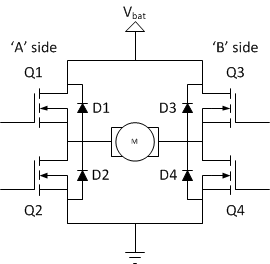
\includegraphics[width=0.5\textwidth]{figs/ch03/h-bridge.png}
        \caption{The load is at the center in an H-like configuration.}
    \end{figure}
    The switching elements (Q1..Q4) are usually bi-polar or FET transistors, in some high-voltage applications IGBTs (insulated-gate bipolar transistor). Integrated solutions also exist but whether the switching elements are integrated with their control circuits or not is not relevant for the most part for this discussion. The diodes (D1..D4) are called catch diodes and are usually of a Schottky type.

    The top-end of the bridge is connected to a power supply (battery for example) and the bottom-end is grounded.

    In general all four switching elements can be turned on and off independently, though there are some obvious restrictions.

    Though the load can in theory be anything you want, by far the most pervasive application if H-bridges is with a brushed DC or bipolar stepper motor (steppers need two H-bridges per motor) load. In the following I will concentrate on applications as a brushed DC motor driver.

    Situations:
    \begin{enumerate}
        \item \textbf{Q1 and Q4 on}: the left lead of the motor will be connected to the power supply, while the right lead is connected to ground. Current starts flowing through the motor which energizes the motor in (let’s say) the forward direction and the motor shaft starts spinning.
        \item \textbf{Q2 and Q4 on}: the reverse will happen, the motor gets energized in the reverse direction, and the shaft will start spinning backwards.
        \item \textcolor{red}{\textbf{Never ever close both Q1 and Q2 (or Q3 and Q4) at the same time}}: you just have created a really low-resistance path between power and GND, effectively short-circuiting your power supply. This condition is called ‘shoot-through’ and is an almost guaranteed way to quickly destroy your bridge, or something else in your circuit.
        \item Table for the 9 different states for the full bridge to be in: 
        \begin{figure}[H]
            \centering
            \begin{tabular}[ H, 0.7\textwidth]{ |c|c|c|c|c|}
                \hline
                    & Q1 & Q2 & Q3 & Q4 \\
                \hline
                    1 & close & open & open & open \\
                \hline
                    2 & close & open & open & close \\
                \hline
                    3 & close & open & close & open \\
                \hline
                    4 & open & close & open & open \\
                \hline
                    5 & open & close & open & close \\
                \hline
                    6 & open & close & close & open \\
                \hline
                    7 & open & open & open & open \\
                \hline
                    8 & open & open & open & close \\
                \hline
                    9 & open & open & close & open \\
                \hline
            \end{tabular}
        \end{figure}
    \end{enumerate}
\end{enumerate}
\label{todo1}  todo this later

\section{DC to DC Converters}
A DC to DC converter converts direct current (DC) electrical power from one voltage level to another. They are essential in many electronic applications where the voltage supplied by batteries or power supplies does not match the voltage required by the electronic components or circuits. The type of DC-DC converter used depends on the application.

\begin{enumerate}
    \item \textbf{Linear regulators}: These are the simplest form of DC-to-DC converters and operate by dissipating excess voltage as heat to maintain a constant output voltage. They are known for their simplicity, low noise output, and fast response to changes in load, but they are inefficient for large differences between input and output voltages because they waste a lot of power as heat.
    \item \textbf{SMPs (switch-mode power supplies)}: These converters use a switching element that turns on and off rapidly, combined with inductors and capacitors, to regulate the output voltage. SMPS are more efficient than linear regulators, especially when there is a significant difference between input and output voltages, because they transfer energy via a switch without dissipating it as heat.The primary types of (SMPs) are:
    \begin{pline}
        \item Buck Converters: Also known as step-down converters, which reduce the input voltage to a lower output voltage
        \item Boost Converters: Also known as step-up converters, they increase the input voltage to a higher output voltage
        \item Buck-Boost Converters: These can either increase or decrease the input voltage depending on the design and requirements
        \item Cuk Converters: Similar to buck-boost converters, these converters differ in that their output reverses polarity, has low ripple current
    \end{pline}
    \begin{figure}[H]
        \centering
        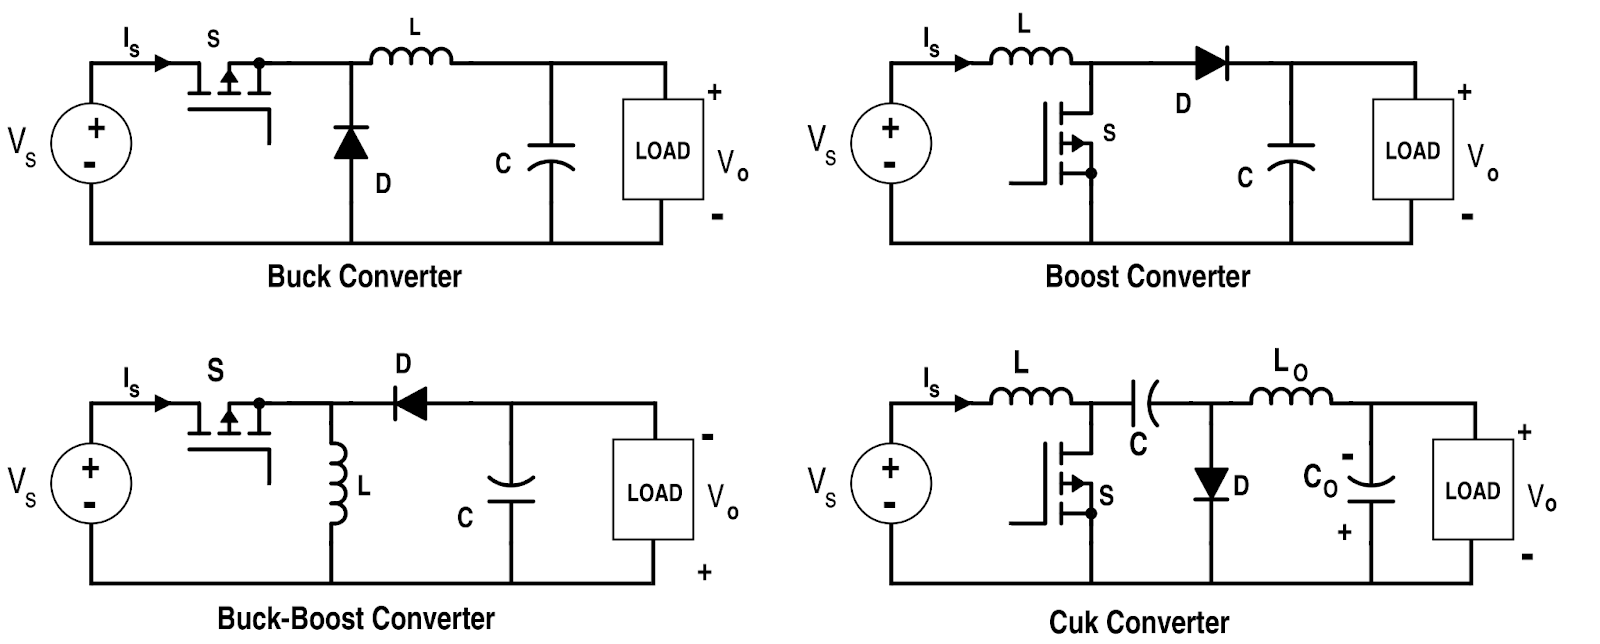
\includegraphics[scale=0.25]{figs/ch03/SMPS.png}
        \caption{Types of SMP converters}
    \end{figure}
    \item \textbf{Isolated converters}: These provide electrical isolation between their input and output, which is critical for safety and noise reduction in sensitive electronic systems. Types of isolated converters include flyback, forward, push-pull, half-bridge, and full-bridge converters. 
\end{enumerate}

\section{AC to DC Converters}
An AC to AC converter is a type of power electronic device that is designed to convert AC electrical power from one waveform to another. This conversion can involve changes in the amplitude, frequency, or phase of the AC signal.

AC to AC converters are used in various applications where the modification of AC power is required. For example, they are essential in applications such as variable-frequency drives for controlling the speed of AC motors, power supplies for devices that require different voltage levels or frequencies than what is provided by the main power grid, and in uninterruptible power supplies (UPS) that may need to regulate and condition the power before delivering it to sensitive equipment.
\begin{enumerate}
    \item \textbf{AC-AC Voltage Controller Converter (AC Choppers)}: AC choppers are a type of converter that directly controls the voltage amplitude of the AC supply without changing the frequency. They achieve this by selectively chopping parts of the input voltage waveform using switches such as thyristors, triacs, or transistors. By controlling the conduction angle or the duration for which the switch is on during each half-cycle of the AC waveform, the average output voltage can be varied. This method is often referred to as phase control. AC choppers are commonly used in light-dimming circuits, speed control of single-phase AC motors, and heating applications. 
    
    \item \textbf{AC Cycloconverter}: Cycloconverters are converters that change the input AC frequency to a lower output frequency without an intermediate DC link. They are essentially direct frequency converters that use controlled semiconductor switches to synthesize the low-frequency output from segments of the input AC waveform. 

    Cycloconverters are mainly classified into two types: step-down cycloconverters, which produce an output frequency lower than the input frequency, and step-up cycloconverters, which are less common due to their complexity and are used to produce a higher output frequency. Cycloconverters are suitable for applications requiring large power and low frequency, such as in driving large motors for rolling mills.

    \item \textbf{Matrix ConverterMatrix Converter}: Matrix converters, direct AC-AC converters, utilize an array of controlled bi-directional switches to connect the input phases to the output phases. Unlike other converters, matrix converters do not require any intermediate energy storage components like capacitors or inductors. The switches are arranged in a matrix form, and by appropriately timing the switching actions, the converter can produce an output voltage with adjustable magnitude and frequency. Matrix converters are capable of bidirectional power flow, which makes them suitable for regenerative braking applications where energy can be fed back into the power supply. They are used in high-performance drive applications, such as machine tools and aircraft power systems. 
    
\end{enumerate}

\section{Sources}
\begin{enumerate}
    \item \href{https://www.quarktwin.com/blogs/converter/understanding-power-converters-a-beginners-guide/459}{Understanding Power Converters : A Beginners Guide}
    \item \href{https://www.rohm.com/electronics-basics/ac-dc/rectification}{Full-Wave Rectification and Half-Wave Rectification}
    \item \href{https://www.rohm.com/electronics-basics/ac-dc/transformer-method}{Transformer Method (AC-DC Converter)}
    \item \href{https://www.rohm.com/electronics-basics/ac-dc/switching-method}{Switching Method (AC-DC Converter)}
    \item \href{https://www.rohm.com/electronics-basics/ac-dc/feedback-control}{Feedback Control}
    \item \href{https://www.rohm.com/electronics-basics/ac-dc/light-load-mode}{Light load mode}
    \item \href{https://www.modularcircuits.com/blog/articles/h-bridge-secrets/h-bridges-the-basics/}{H-bridges - the basics}
\end{enumerate}